\begin{frame}{Existent solutions}
	
	\pause
	\begin{itemize}
		\item Long short-term memory (LSTM). Hochreiter, Schmidhuber (1997) \cite{lstm}
			\begin{itemize}
				\item the network structure is modified with specialized "memory cells"
				\item a truncated version of back-propagation is employed
			\end{itemize}
		\pause
		\item Hessian-Free optimization (HF). Martens (2010) \cite{hessianFree}
		\begin{itemize}
			\item a second order method
			\item a "cheap" approximation of the Hessian is employed
			\item the quadratic sub-problem is solved through conjugate gradient + structural damping
		\end{itemize}
		\pause
		\item Pascanu, Bengio (2013) \cite{pascanu}
		\begin{itemize}
			\item a first order method
			\item uses a penalty to deal with the vanishing gradient problem
		\end{itemize}
	\end{itemize}
	
\end{frame}

\begin{frame}{Understanding the gradient structure: unfolding}
	\tikzstyle{rnn_style}=[->,shorten >=1pt,auto,node distance=1.5cm,
	thick,
	neuron/.style={circle,fill=white!50,draw,minimum size=0.7cm,font=\sffamily\Large\bfseries},
	missing/.style={circle,fill=white!50,draw=none,minimum size=0.7cm,font=\sffamily\Huge\bfseries},
	label/.style={node distance=1.2cm,rectangle,fill=white!50,draw=none,minimum size=0.7cm,font=\sffamily\normalsize},
	layer/.style={rectangle,fill=white!50,draw,minimum width=4cm,font=\sffamily\normalsize},
	loopStyle/.style={in=120,out=60, distance=2.5cm},]
	
	
	
	\begin{figure}[h!]
		\centering
		\resizebox{8cm}{!}{
			\begin{tikzpicture}[rnn_style]
			
			%t=0
			\node[layer] (hl1) {Hidden layer t=0};
			
			\node[neuron]    (x0)[below left=0.3cm and 1cm of hl1]       {};
			\node[label]    (u0)[left of=x0]   {$\vec{u}_1$};
			
			
			
			\node[neuron] (o0) [above right=0.3cm and 1cm of hl1] {};
			\node[label]    (y0)[right of=o0]   {$\vec{y}_1$};
			
			%t=1
			\node[layer] (hl2)[above of=hl1,node distance=2.5cm] {Hidden layer t=1};
			
			\node[neuron]    (x1)[below left=0.3cm and 1cm of hl2]      {};
			\node[label]    (u1)[left of=x1]   {$\vec{u}_2$};
			
			
			\node[neuron] (o1) [above right=0.3cm and 1cm of hl2] {};
			\node[label]    (y1)[right of=o1]   {$\vec{y}_2$};
			
			%dots
			\node[label,font=\sffamily\Huge\bfseries] (hld)[above of=hl2,node distance=2cm] {$\hdots$};
			
			%t=T
			\node[layer] (hlT)[above of=hld,node distance=2cm] {Hidden layer t=T};
			
			\node[neuron]    (xT)[below left=0.3cm and 1cm of hlT]      {};
			\node[label]    (uT)[left of=xT]   {$\vec{u}_T$};
			
			
			\node[neuron] (oT) [above right=0.3cm and 1cm of  hlT] {};
			\node[label]    (yT)[right of=oT]   {$\vec{y}_T$};
			
			
			%biases
			\node[neuron](b) [right of=y1,node distance=1.4cm] {};
			\node[label] (b_l) [above of=b,node distance=0.7cm] {bias=1};
			
			
			\path[->] (x0) edge [bend right] node[]{$W^{in}$}   (hl1)
			(u0) edge []   (x0)
			(o0) edge []   (y0)
			(x1) edge [bend right] node[]{$W^{in}$} (hl2)
			(u1) edge []   (x1)
			(o1) edge []   (y1)
			(xT) edge [bend right] node[]{$W^{in}$} (hlT)
			(uT) edge []   (xT)
			(oT) edge []   (yT)
			
			
			(hl1) edge [bend left]  node[]{$W^{out}$} (o0)
			(hl2) edge [bend left]  node[]{$W^{out}$} (o1)
			(hlT) edge [bend left]  node[]{$W^{out}$} (oT)
			
			(b)  edge [bend left,dotted,in = 90]  node[]{$b^{out}$} (o0)
			(b)  edge [bend left, dotted, in = 90,out=80]  node[]{$b^{rec}$} (hl1)
			(b)  edge [bend left, dotted]  node[]{$b^{rec}$} (hl2)
			(b)  edge [bend left,dotted]  node[]{$b^{out}$} (o1)
			(b)  edge [bend left, dotted,in = 200]  node[]{$b^{rec}$} (hlT)
			(b)  edge [bend left,dotted,in =200]  node[]{$b^{out}$} (oT)
			(hl1) edge [] node[]{$W^{rec} $} (hl2)
			(hl2) edge [] node[]{$W^{rec} $} (hld)
			(hld) edge [] node[]{$W^{rec} $} (hlT);
			
			\end{tikzpicture}
		}
		\caption{Unfolding of a $\net{RNN}$}
		\label{rnn_unfolding}
	\end{figure}
\end{frame}

\begin{frame}{Understanding the gradient structure}
	It's easy to see that
	\begin{equation}
	\nabla L(\vec{x}) = \sum_{t=1}^T \nabla L_{|t}(\vec{x}),
	\end{equation}
	where $\nabla L_{|t}$ is ...
\end{frame}

\begin{frame}{Temporal gradient norms: an illustration}
	\begin{figure}
		\centering
		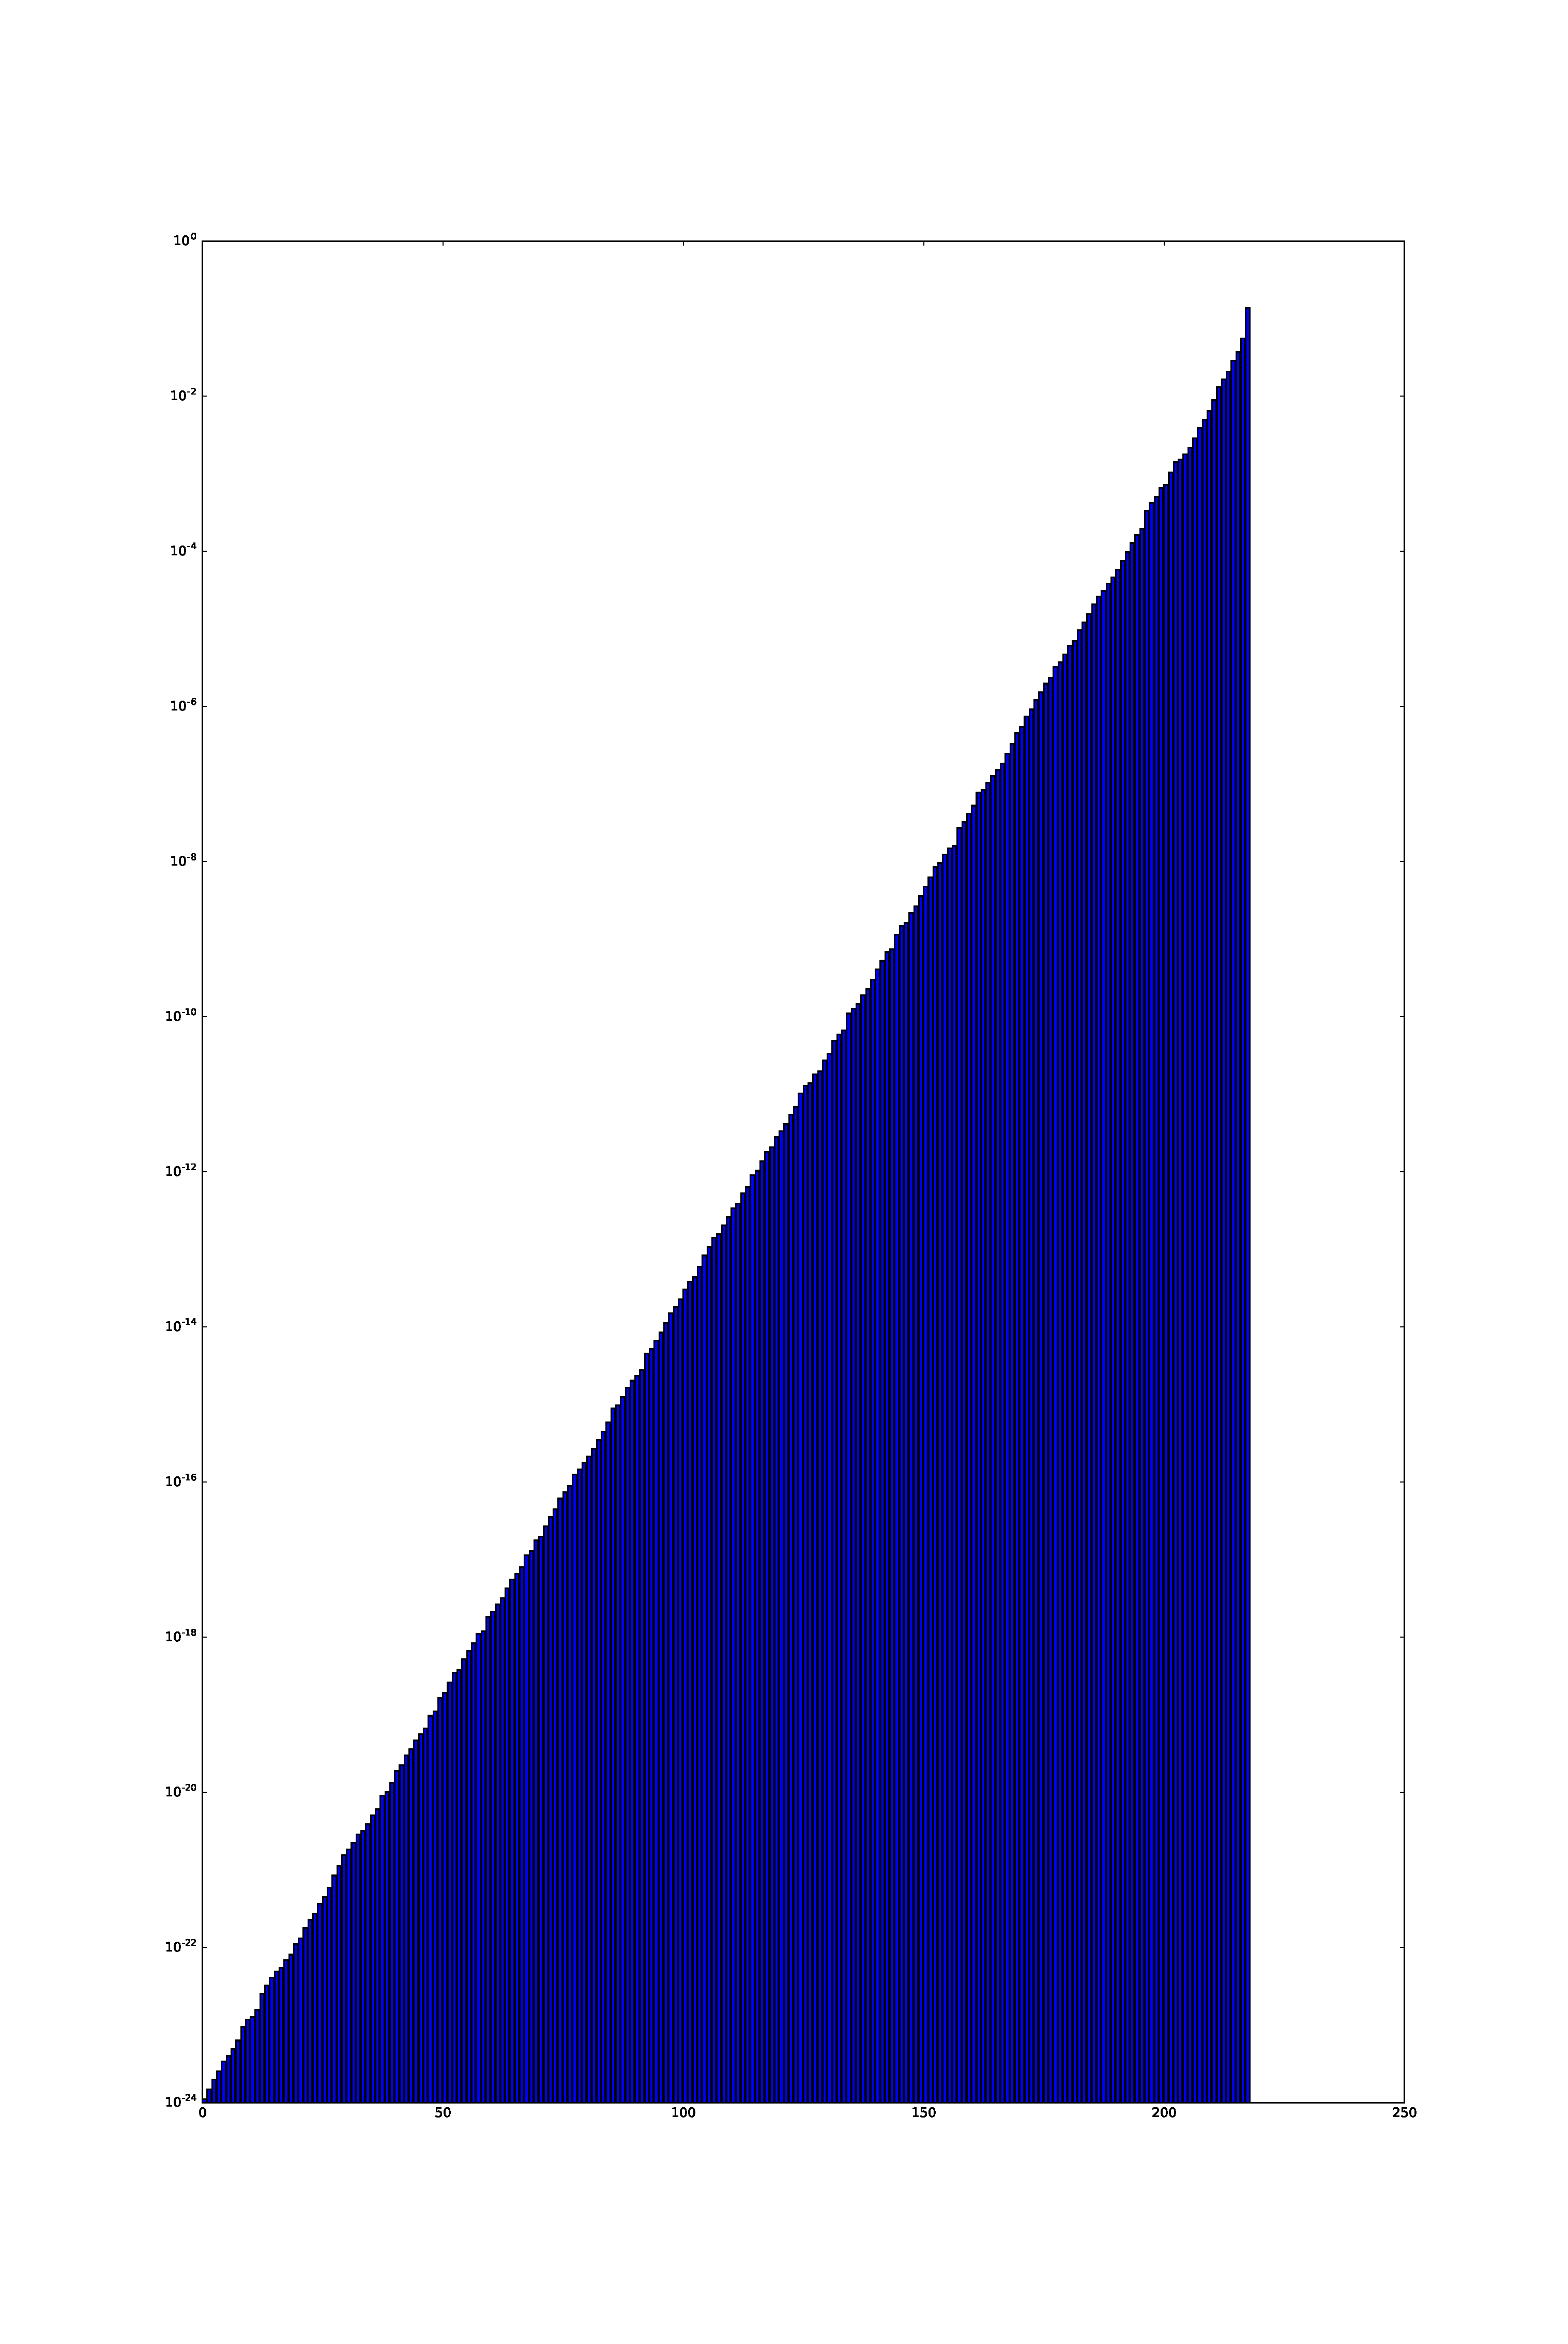
\includegraphics[width=1\textwidth]{temporal_gradients.eps}
	\end{figure}
\end{frame}


\begin{frame}{A new proposal}
\begin{itemize}
	\item use the structure of the gradient to compute a descent direction which does not suffer from the vanishing gradient problem
	
	\item normalize the temporal components
	\begin{equation}
	d(\vec{x}) = \sum_{t=1}^T \frac{\nabla L_{|t}(\vec{x})}{\norm{\nabla L_{|t}(\vec{x})}}
	\end{equation}
	
	\item add some randomness for robustness:
		\begin{equation}
		d(\vec{x}) = \sum_{t=1}^T \beta_t\frac{\nabla L_{|t}(\vec{x})}{\norm{\nabla L_{|t}(\vec{x})}},
		\end{equation}
		
		with $\sum_{t=1}^T\beta_t=1, \beta_t>0$
\end{itemize}



\end{frame}
